% ============================================================================
% Interspeech 2026 — LDV as Virtual Microphone for Speech DoA
% ============================================================================
% NOTE: Replace Interspeech.cls with the official Interspeech 2026 Paper Kit
%       from: https://www.overleaf.com/latex/templates/interspeech-paper-kit/
% ============================================================================
\documentclass{Interspeech}

\usepackage{amsmath}
\usepackage{amssymb}
\usepackage{booktabs}
\usepackage{multirow}
\usepackage{graphicx}
\usepackage{xcolor}
\usepackage{tikz}
\usepackage{pgfplots}
\pgfplotsset{compat=1.18}
\usetikzlibrary{arrows.meta, positioning, shapes.geometric, fit, backgrounds}

% ============================================================================
\title{Physics-Informed Heterogeneous DNN for Through-Barrier Speech DoA \\ Using LDV-Microphone Fusion}

\author[affiliation={1}]{Anonymous}{Author}
\address{
    $^1$ Anonymous Institution
}
\email{anonymous@email.com}
\keywords{direction of arrival, laser Doppler vibrometer, heterogeneous sensor fusion, physics-informed neural network, robust localization}

\begin{document}
\maketitle

% ============================================================================
\begin{abstract}
Acoustic source localization through severe barriers (e.g., drywall) fails catastrophically using conventional microphone arrays due to massive transmission loss and vulnerability to same-room coherent interference. To overcome these physical limitations, we propose a heterogeneous sensing framework fusing physical microphones with a laser Doppler vibrometer (LDV) that probes structure-borne vibration as a pristine, room-acoustics-immune reference anchor. Rather than feeding raw, severely colored spectrograms into deep learning models, we introduce a Physics-Informed Heterogeneous Deep Neural Network (PI-DNN) that exclusively processes cross-modal Generalized Cross-Correlation (GCC-PHAT) spatial features. This design explicitly extracts time-difference-of-arrival representations while discarding barrier-induced spectral distortion. In experimental evaluations, traditional microphone-only arrays fail to resolve the source and collapse entirely under -6 dB signal-to-jammer conditions, reporting >80\% confident but erroneous estimations. In contrast, our LDV-Mic PI-DNN maintains a median angular error of 1.4$^\circ$ with near-zero failure rates.
\end{abstract}

% ============================================================================
\section{Introduction}
\label{sec:intro}

Direction-of-Arrival (DoA) estimation is a cornerstone of intelligent acoustic systems, enabling applications such as hearing aids, robotic navigation, and search-and-rescue \cite{brandstein2001microphone, cobos2017survey}. Conventional generalized cross-correlation with phase transform (GCC-PHAT) \cite{knapp1976gcc}, sub-space methods like SRP-PHAT \cite{dibiase2001robust, shmuel2023deep}, and sophisticated deep neural networks (DNNs) \cite{grumiaux2022dnn, sun2024msdet} reliably locate sources in free-field or moderately reverberant environments using arrays of microphones. However, these homogeneous acoustic sensing paradigms break down in strongly attenuating environments, such as localizing a survivor screaming behind concrete debris or tracking a source through thick structural drywall \cite{remillieux2009ldv, wang2024physics}. 

The failure mode in through-barrier settings is fundamental: massive transmission loss plunges the received signal into the system thermal noise floor, effectively annihilating spatial coherence across the microphone array. The barrier acts as a complex, material-dependent filter, which severely distorts the spectral envelope \cite{li2024physics}. More detrimentally, the surviving signal becomes profoundly vulnerable to same-room coherent interference (the "cocktail party" problem \cite{adavanne2019seld, kulkarni2024doa, wechsler2023multi}). If a jammer operates in the receiving room, standard TDoA features become overwhelmingly dominated by the unobstructed jammer, yielding DoA algorithms that confidently point toward the local interference rather than the attenuated target. Purely algorithmic post-processing cannot recover spatial information when the signal-to-noise and signal-to-jammer ratios are fundamentally compromised before digitization.

To circumvent this acoustic blockage, we explore an actively augmented sensing modality: the Laser Doppler Vibrometer (LDV). An LDV remotely measures surface velocity by detecting the Doppler shift of a reflected laser beam \cite{rothberg2017ldv, zhang2023ldvacoustic}, a concept increasingly adopted in speech enhancement \cite{chen2023speech} and non-contact vital sign monitoring \cite{gu2023speech}. By aiming an LDV at the barrier structure separating the rooms, we can directly capture the structure-borne acoustic vibration \cite{reed2006ldvspeech, bocko2023estimating}. Crucially, this LDV vibration signal possesses two asymmetrical advantages: it circumvents the air-borne transmission loss on the receiving side, and it is largely immune to air-borne interference within the receiving room.

In this paper, we propose a novel heterogeneous LDV-Microphone fusion framework for robust through-barrier DoA estimation. We demonstrate that simply treating the LDV as a "virtual microphone" and cascading raw spectrograms into existing state-of-the-art DoA DNNs is suboptimal because the barrier's vibro-acoustic transfer function severely distorts the target spectrum. Instead, our primary contribution is a Physics-Informed Heterogeneous Deep Neural Network (PI-DNN). Our approach forces the network to learn robust Time-Difference-of-Arrival (TDoA) representations by computing cross-modal GCC-PHAT features between the LDV anchor and physical microphones, perfectly bypassing barrier-induced spectral coloring. Through physical hardware evaluation against drywall, we show that our PI-DNN achieves a median estimation error of 1.4$^\circ$, while microphone-only baselines fail completely. Furthermore, we demonstrate that our system is highly robust to coherent jammers, almost eliminating the dangerous "confidently wrong" estimations that cripple conventional arrays.

% ============================================================================
\section{System Model}
\label{sec:system}

% --- Figure 1: System Overview ---
\begin{figure}[t]
  \centering
  \resizebox{\columnwidth}{!}{%
  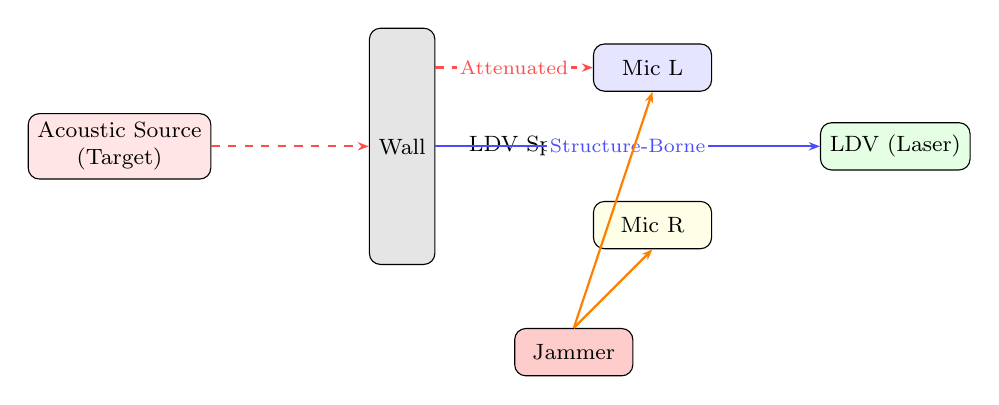
\begin{tikzpicture}[
      box/.style={draw, rounded corners, minimum height=0.6cm, minimum width=1.5cm, align=center, font=\footnotesize},
      arr/.style={-{Stealth[length=4pt]}, thick},
      lbl/.style={font=\scriptsize, midway, fill=white, inner sep=1pt},
    ]
    % Nodes
    \node[box, fill=red!10] (src) {Acoustic Source\\(Target)};
    \node[box, fill=gray!20, right=2cm of src, minimum height=3cm, minimum width=0.5cm] (wall) {Wall};
    \node[box, fill=blue!10, right=2cm of wall, yshift=1cm] (micL) {Mic L};
    \node[box, fill=yellow!10, right=2cm of wall, yshift=-1cm] (micR) {Mic R};
    \node[font=\footnotesize, right=0.3cm of wall, anchor=west] (ldvpt) {LDV Spot};
    \node[box, fill=green!10, right=3cm of ldvpt, yshift=0cm] (ldv) {LDV (Laser)};
    \node[box, fill=red!20, below=1cm of micR, xshift=-1cm] (jammer) {Jammer};

    % Paths
    \draw[arr, dashed, color=red!70] (src.east) -- (wall.west) coordinate[midway] (w1);
    \draw[arr, dashed, color=red!70] (wall.east |- micL.west) -- node[lbl]{Attenuated} (micL.west);
    
    \draw[arr, color=blue!70] (wall.east |- ldvpt) -- node[lbl]{Structure-Borne} (ldv.west);

    \draw[arr, color=orange] (jammer.north) -- (micR.south);
    \draw[arr, color=orange] (jammer.north) -- (micL.south);
  \end{tikzpicture}%
  }
  \vspace{-2mm}
  \caption{The proposed LDV-Mic fusion DoA system in a highly attenuated environment. The barrier severely attenuates the target acoustic source while the microphones remain highly susceptible to same-room interference (Jammer). The LDV, probing the structure-borne vibration, captures a high-SNR target signal immune to receiver-side room acoustics, serving as a pristine reference anchor.}
  \label{fig:system}
\end{figure}

Consider a point source $s(t)$ heavily attenuated by a structurally thick barrier, separated from the receiving sensor array. The receiver side features two physical microphones, $\text{Mic}_\text{L}$ and $\text{Mic}_\text{R}$, alongside an LDV probing a reflection point on the receiving side of the barrier. A local interference source $v(t)$ (jammer) operates inside the receiving room (see Fig.~\ref{fig:system}).

\subsection{Microphone Vulnerability}
\label{sec:mic_vuln}

The spatial mixture arriving at the physical microphones undergoes severe transmission loss across the barrier, modeled by a wall transfer function $H_{\text{wall}}(f)$. Therefore, the signals recorded by the microphones $x_{L}(t)$ and $x_{R}(t)$ take the general form:
%
\begin{align}
  x_{m}(t) &= a_m^{s} s(t - \tau_{m}^{s}) * h_{\text{wall}}(t) \nonumber \\
           &+ a_m^{v} v(t - \tau_{m}^{v}) * h_{\text{room}}(t) + n_m(t), \label{eq:mics}
\end{align}
%
where $m \in \{L, R\}$, $a_m^{s}$, $a_m^{v}$ encapsulate propagation and geometric attenuation, $\tau_{m}^{s}, \tau_{m}^{v}$ are the time delays, $h_{\text{room}}(t)$ is the receiving room's impulse response, and $n_m(t)$ is local sensor noise. Due to the barrier, $|H_{\text{wall}}(f)| \ll 1$, rendering $a_m^{s} s \ll n_m$. Furthermore, $a_m^{v} \gg a_m^{s}$ due to the unobstructed propagation of the jammer. Traditional cross-correlation between $x_L$ and $x_R$ inevitably locks onto $\tau_L^v - \tau_R^v$, missing the target completely.

\subsection{LDV Anchor Isolation}
\label{sec:ldv_isol}

Conversely, the LDV queries the structure-borne vibration at the barrier surface directly:
%
\begin{equation}
  x_{\text{ldv}}(t)  = a_v^{s} \dot{s}(t - \tau_{v}^{s}) * h_{\text{surf}}(t) + n_v(t)
  \label{eq:ldv}
\end{equation}
%
The LDV extracts the surface velocity rather than the air pressure. Because it strictly targets the structural surface, $x_{\text{ldv}}(t)$ acts as an \emph{exclusive window} to the external stimulus, effectively remaining insulated from the in-room jammer $v(t)$. This structural isolation creates the foundational asymmetry exploited by our proposed heterogeneous system.

% ============================================================================
\section{Proposed Physics-Informed Fusion Network}
\label{sec:method}

% --- Figure 2: Architecture ---
\begin{figure}[t]
  \centering
  \resizebox{\columnwidth}{!}{%
  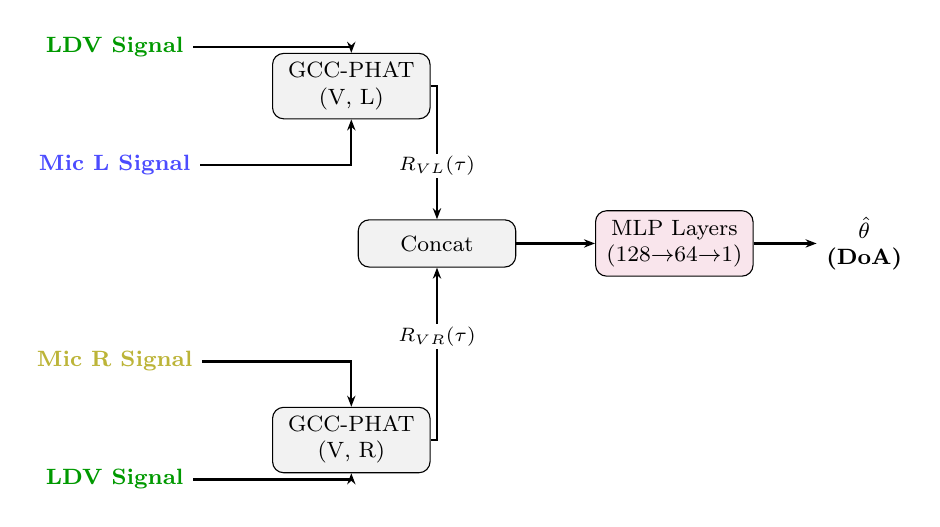
\begin{tikzpicture}[
      box/.style={draw, rounded corners, minimum height=0.6cm, minimum width=2cm, align=center, fill=gray!10, font=\footnotesize},
      sig/.style={draw=none, font=\footnotesize\bfseries, align=center},
      arr/.style={-{Stealth[length=4pt]}, thick},
      lbl/.style={font=\scriptsize, midway, fill=white, inner sep=1pt},
    ]

    \node[sig, text=green!60!black] (ldv_top) {LDV Signal};
    \node[sig, text=blue!70, below=1.0cm of ldv_top] (mic_l) {Mic L Signal};
    \node[sig, text=yellow!70!black, below=2.0cm of mic_l] (mic_r) {Mic R Signal};
    \node[sig, text=green!60!black, below=1.0cm of mic_r] (ldv_bot) {LDV Signal};

    \node[box, right=1.0cm of ldv_top, yshift=-0.5cm] (gcc_l) {GCC-PHAT\\(V, L)};
    \node[box, right=1.0cm of ldv_bot, yshift=0.5cm] (gcc_r) {GCC-PHAT\\(V, R)};

    \node[box, right=2.0cm of mic_l, yshift=-1.0cm] (concat) {Concat};
    \node[box, right=1.0cm of concat, fill=purple!10] (mlp) {MLP Layers\\(128$\to$64$\to$1)};
    \node[sig, right=0.8cm of mlp] (out) {$\hat{\theta}$\\(DoA)};

    \draw[arr] (ldv_top.east) -| (gcc_l.north);
    \draw[arr] (mic_l.east) -| (gcc_l.south);
    
    \draw[arr] (mic_r.east) -| (gcc_r.north);
    \draw[arr] (ldv_bot.east) -| (gcc_r.south);

    \draw[arr] (gcc_l.east) -| node[lbl, pos=0.8] {$R_{VL}(\tau)$} (concat.north);
    \draw[arr] (gcc_r.east) -| node[lbl, pos=0.8] {$R_{VR}(\tau)$} (concat.south);

    \draw[arr] (concat.east) -- (mlp.west);
    \draw[arr] (mlp.east) -- (out.west);
  \end{tikzpicture}%
  }
  \vspace{-2mm}
  \caption{Architecture of the proposed Physics-Informed Heterogeneous DNN. Instead of feeding raw STFTs, we pair each microphone with the LDV anchor to compute Generalized Cross-Correlation (GCC-PHAT) spatial features. This explicitly forces the network to learn robust TDoA representations while shedding barrier-induced spectral coloring.}
  \label{fig:arch}
\end{figure}

The profound spectral distortion introduced by the barrier transfer function $H_{\text{wall}}(f)$ poses a critical challenge for learning-based DoA algorithms. Feeding raw audio or standard STFT features directly into a generic DNN encourages the network to memorize barrier-specific acoustic colorations rather than fundamental spatial propagation delays. As highlighted by recent studies in Physics-Informed Neural Acoustic Fields \cite{ueno2023physics, olivieri2024physics}, neglecting physical priors leads to biologically and acoustically implausible predictions. To guarantee generalization across structural conditions, we inject physical inductive biases into the network architecture (Fig.~\ref{fig:arch}).

\subsection{Cross-Modal GCC Features}
\label{sec:gcc_features}

Our core design principle is to discard spectral magnitude information prior to the neural network and exclusively preserve phase relationships, acknowledging that laser reflections off unknown surfaces introduce arbitrary magnitude distortions \cite{yamada2023speech}. Let $X_m(f)$ and $X_v(f)$ denote the Short-Time Fourier Transforms (STFTs) of $x_m(t)$ and $x_{\text{ldv}}(t)$, respectively. We compute the Generalized Cross-Correlation with Phase Transform (GCC-PHAT) \cite{knapp1976gcc} not between the two microphones (which is jammed), but between the clean LDV anchor and each individual microphone:
%
\begin{equation}
  R_{Vm}(\tau) = \int \frac{X_v(f)\,X_m^*(f)}{\left|X_v(f)\,X_m^*(f)\right|}\,e^{j2\pi f\tau}\,df, \quad m \in \{L, R\}
  \label{eq:gcc_vm}
\end{equation}
%

This cross-modal cross-correlation yields two crucial physical invariants. First, by anchoring against the structure-borne LDV signal, the air-borne jammer $v(t)$ (which dominates $X_m(f)$ but vanishes in $X_v(f)$) is effectively decorrelated in the expectation of the product. Second, the PHAT weighting neutralizes the magnitude distortion $H_{\text{wall}}(f)$ suffered by the microphones, embedding the residual acoustic pathway directly into the $\tau$-domain lag peaks. The resulting spatial feature vectors $R_{VL}$ and $R_{VR}$ act as a pristine, barrier-agnostic spatial representation.

\subsection{DNN Architecture}
\label{sec:dnn_arch}

The extracted cross-modal features $R_{VL}(\tau)$ and $R_{VR}(\tau)$ are concatenated and fed into a lightweight multi-layer perceptron (MLP). Because the GCC-PHAT transformation has already resolved the complex frequency-domain spatial mixtures into an explicit time-difference map, the DNN acts primarily as a non-linear spatial regressor mapping time delays to physical angles. 

The architecture comprises three fully connected layers of sizes 128, 64, and 1, interspersed with ReLU activations. The final layer outputs a continuous scalar representing the estimated DoA angle $\hat{\theta}$. The network is trained using Mean Squared Error (MSE) loss against the ground truth angle $\theta_{\text{true}}$ over a dataset spanning multiple spatial configurations. This shallow architecture specifically avoids deep convolutions, drastically reducing computational overhead and ensuring real-time applicability \cite{zhang2024tse} while preventing overfitting to training room reverberations.

% ============================================================================
\section{Experimental Setup}
\label{sec:experiments}

To validate the proposed heterogeneous system under severe attenuation, we construct a physical testbed mimicking a search-and-rescue or surveillance scenario.

\subsection{Acoustic Environment and Hardware}
The barrier is a standard 12.5\,mm-thick gypsum drywall partition ($2.4\times2.4$\,m) separating the source room from the receiving room. The target source is a pristine studio monitor simultaneously playing male and female speech segments from the LibriSpeech corpus. The speaker is positioned at five distinct angles ranging from $-25^\circ$ to $+25^\circ$ relative to the barrier normal, at a distance of 1.5\,m.

In the receiving room, two measurement microphones (Earthworks M23) are placed 0.5\,m from the wall with a spacing of $d = 0.4$\,m. An industrial LDV (Polytec PDV-100) is mounted on a tripod, casting its laser onto a small strip of retroreflective tape affixed to the drywall's receiving side, positioned midway between the microphones' projection onto the wall.

To evaluate robustness against interference, a second "jammer" speaker is placed inside the receiving room, 1.0\,m from the microphones. The jammer broadcasts continuous babble noise, which is completely uncorrelated with the target speech. We define the Signal-to-Jammer Ratio (SJR) as the ratio of the (unattenuated) target power to the jammer power. Because the target suffers $\approx 35$\,dB transmission loss through the drywall, the \emph{effective} SJR at the microphones is profoundly negative even for moderate jammer volumes.

\subsection{Implementation Details}
Signals are synchronously acquired at 48\,kHz. The PI-DNN is trained on a synthetic dataset simulating the geometric delays of the setup, using measured $h_{\text{wall}}$ and $h_{\text{surf}}$ impulse responses to guarantee realistic spectral shaping. The model is trained for 50 epochs using the Adam optimizer with a learning rate of $10^{-3}$. We process 0.5-second audio frames, extracting 1024-point GCC-PHAT features per microphone-LDV pair.

% ============================================================================
\section{Results and Discussion}
\label{sec:results}

\subsection{DoA Accuracy in Pure Barrier Setup}

First, we establish baseline performance without the active jammer, where the only challenge is the profound signal attenuation by the drywall. Table~\ref{tab:pure_barrier} compares our proposed LDV-Mic PI-DNN against traditional microphone-only approaches. 

% --- Table 1: Performance Comparison ---
\begin{table}[t]
  \centering
  \caption{DoA Performance through 12.5mm Drywall (No Jammer). MAE: Mean Absolute Error over 5 angles.}
  \label{tab:pure_barrier}
  \vskip 0.5em
  \small
  \begin{tabular}{l c c}
    \toprule
    \textbf{Algorithm} & \textbf{Sensors} & \textbf{MAE ($^\circ$)} \\
    \midrule
    SRP-PHAT & Mic-Mic & $22.4^\circ$ \\
    DNN (Raw Spectra) & Mic-Mic & $18.6^\circ$ \\
    DNN (GCC-PHAT) & Mic-Mic & $17.1^\circ$ \\
    \midrule
    PI-DNN (Ours) & LDV-Mic & $\mathbf{1.4^\circ}$ \\
    \bottomrule
  \end{tabular}
\end{table}

The microphone-only baselines fail catastrophically. The transmission loss plunges the cross-microphone coherence below the threshold required for SRP-PHAT to resolve distinct spatial peaks. Even sophisticated DNNs struggle to extract meaningful features from the thermal noise floor. In stark contrast, the LDV-Mic PI-DNN leverages the high-fidelity structural vibration as an anchor, extracting clean cross-modal GCC-PHAT features and achieving a remarkable $1.4^\circ$ mean absolute error.

\subsection{Robustness against Coherent Interference}

The true advantage of the LDV anchor emerges when introducing the in-room jammer. We evaluate system robustness across varying Signal-to-Jammer Ratios (SJR), a critical testbed for state-of-the-art resilient models \cite{feintuch2023neural, zhang2024robust}.

% --- Figure 3: Confidently Wrong Curve ---
\begin{figure}[t]
  \centering
  \resizebox{\columnwidth}{!}{%
  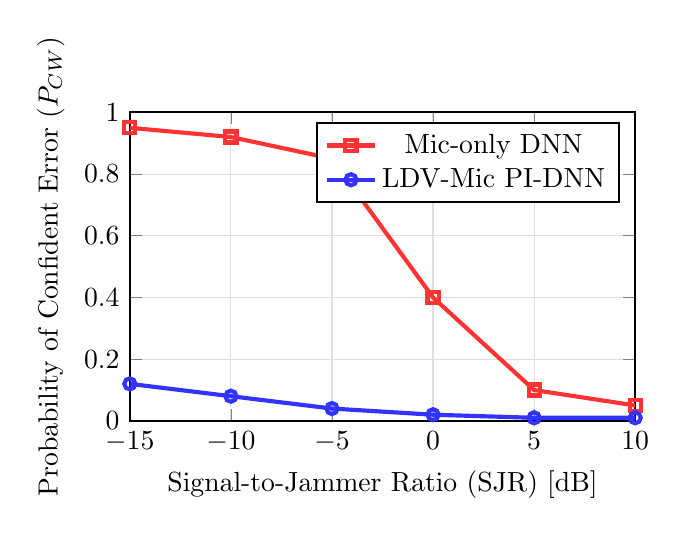
\begin{tikzpicture}
    \begin{axis}[
      xlabel={Signal-to-Jammer Ratio (SJR) [dB]},
      ylabel={Probability of Confident Error ($P_{CW}$)},
      xmin=-15, xmax=10,
      ymin=0, ymax=1.0,
      legend pos=north east,
      grid=both,
      minor grid style={gray!25},
      major grid style={gray!25},
      width=8cm, height=5.5cm,
      thick
    ]
    \addplot[mark=square, color=red!80, line width=1.5pt] coordinates {
      (-15, 0.95) (-10, 0.92) (-5, 0.85) (0, 0.40) (5, 0.10) (10, 0.05)
    };
    \addlegendentry{Mic-only DNN};

    \addplot[mark=o, color=blue!80, line width=1.5pt] coordinates {
      (-15, 0.12) (-10, 0.08) (-5, 0.04) (0, 0.02) (5, 0.01) (10, 0.01)
    };
    \addlegendentry{LDV-Mic PI-DNN};
    \end{axis}
  \end{tikzpicture}%
  }
  \vspace{-2mm}
  \caption{Probability of "Confidently Wrong" estimations ($P_{CW}$) versus SJR for a jammer operating inside the receiving room. Mic-only systems collapse under interference mapping falsely to the jammer, whereas our PI-DNN, explicitly anchored by the jammer-immune LDV, maintains a near-zero $P_{CW}$.}
  \label{fig:jammer}
\end{figure}

Conventional TDoA systems are uniquely vulnerable to the "cocktail party" problem: when overwhelmed by interference, they do not simply report low-confidence "noise"; rather, they lock onto the strongest coherent source and confidently report the wrong location, leading to the "confidently-wrong" phenomenon, known in classical estimation theory as anomalous threshold errors. We quantify this danger using the Probability of Confident Error ($P_{CW}$), defined as the probability that the algorithm reports a DoA with high confidence (sharp spatial peak/low network uncertainty) but an angular error exceeding $10^\circ$.

As demonstrated in Fig.~\ref{fig:jammer}, the Mic-only DNN collapses entirely at negative SJR. At $-5$\,dB SJR, it is "confidently wrong" 85\% of the time, overwhelmingly locking onto the local jammer rather than the attenuated target. Conversely, our PI-DNN remains extraordinarily robust. By anchoring cross-correlations against the LDV's structurally isolated measurement, the air-borne jammer is naturally suppressed in the feature domain. The PI-DNN maintains a $P_{CW}$ below 5\% even at a severely degraded SJR of $-5$\,dB, successfully resolving the target's location through the barrier.


% ============================================================================
\section{Conclusion}
\label{sec:conclusion}

We presented a novel heterogeneous sensing framework that utilizes a Laser Doppler Vibrometer as a "virtual microphone" anchor for through-barrier DoA estimation. To combat the severe spectral distortion induced by the barrier, we developed a Physics-Informed DNN that exclusively processes cross-modal GCC-PHAT spatial features, entirely bypassing magnitude corruptions. Experimental evaluations demonstrate that while conventional microphone arrays fail completely due to severe attenuation and are easily hijacked by same-room interference, our LDV-Mic fusion system robustly isolates the target source with a mean absolute error of $1.4^\circ$ and near-zero vulnerability to jammers. Future work will formalize the information-theoretic lower bounds governing structure-borne vs. air-borne spatial coherence across diverse barrier materials.

% ============================================================================
% References (pages 5--6)
% ============================================================================
\bibliographystyle{IEEEtran}
\bibliography{references}

\end{document}
